\chapter{Methodology}
\label{ch:methodology}

\section{Data}
\label{sec:data}

All numbers in this section are produced by \texttt{scripts/eda\_data\_layers.py}; the full
tables are kept in \texttt{docs/eda/data-layers.md}. Prices are in absolute VND.

\subsection{Sources}

Two daily price layers were built for the \gls{hose} equity market.

\begin{description}
  \item[Layer A] The \gls{ssi} FastConnect Data \gls{api} (\texttt{DailyStockPrice}), pulled
    market-wide in 30-day windows. It returns, for every listed instrument and session, raw
    \gls{ohlcv}, the exchange's reference, ceiling and floor prices, an adjusted close, matched
    and put-through volume, and foreign buy/sell flow. Because each window is queried by date
    rather than by ticker, stocks that were later delisted or moved to another exchange are
    included: the layer is free of survivorship bias. History starts in 2020; in practice the
    cross-section is complete from \textbf{26 February 2020} (one ticker before that date).
  \item[Layer B] A one-pass refetch of adjusted daily bars from a third-party vendor (VCI, via
    the parent research project), 2013--2026. It is longer, but it only holds tickers that were
    still listed when it was fetched and it carries no raw prices, limit prices or foreign flow.
\end{description}

The two layers are not spliced into one series. They use different adjustment conventions
(Section~\ref{sec:data-adjustment}), so joining them would put a seam at the splice date.

\subsection{Coverage}

Table~\ref{tab:data-layers} compares the two layers and Figure~\ref{fig:data-coverage} shows
the number of stocks covered each year.

\begin{table}[ht]
  \centering
  \caption{Daily data layers for \acrshort{hose} stocks.}
  \label{tab:data-layers}
  \begin{tabular}{lrr}
    \toprule
                                          & Layer A (SSI)     & Layer B (VCI)     \\
    \midrule
    Period                                & 2020-02 -- 2026-10 & 2013 -- 2026-10   \\
    Stocks                                & 448               & 308               \\
    Stock-sessions                        & 648{,}901         & 861{,}923         \\
    Delisted / moved stocks included      & 36                & 0                 \\
    Raw prices, reference/limit prices    & yes               & no                \\
    Foreign flow                          & yes               & no                \\
    Median bar completeness$^{a}$         & 1.000 (p5 0.995)  & 1.000 (p5 0.971)  \\
    \bottomrule
  \end{tabular}

  \smallskip
  {\footnotesize $^{a}$ Bars per stock divided by exchange sessions between its first and last bar.}
\end{table}

\begin{figure}[ht]
  \centering
  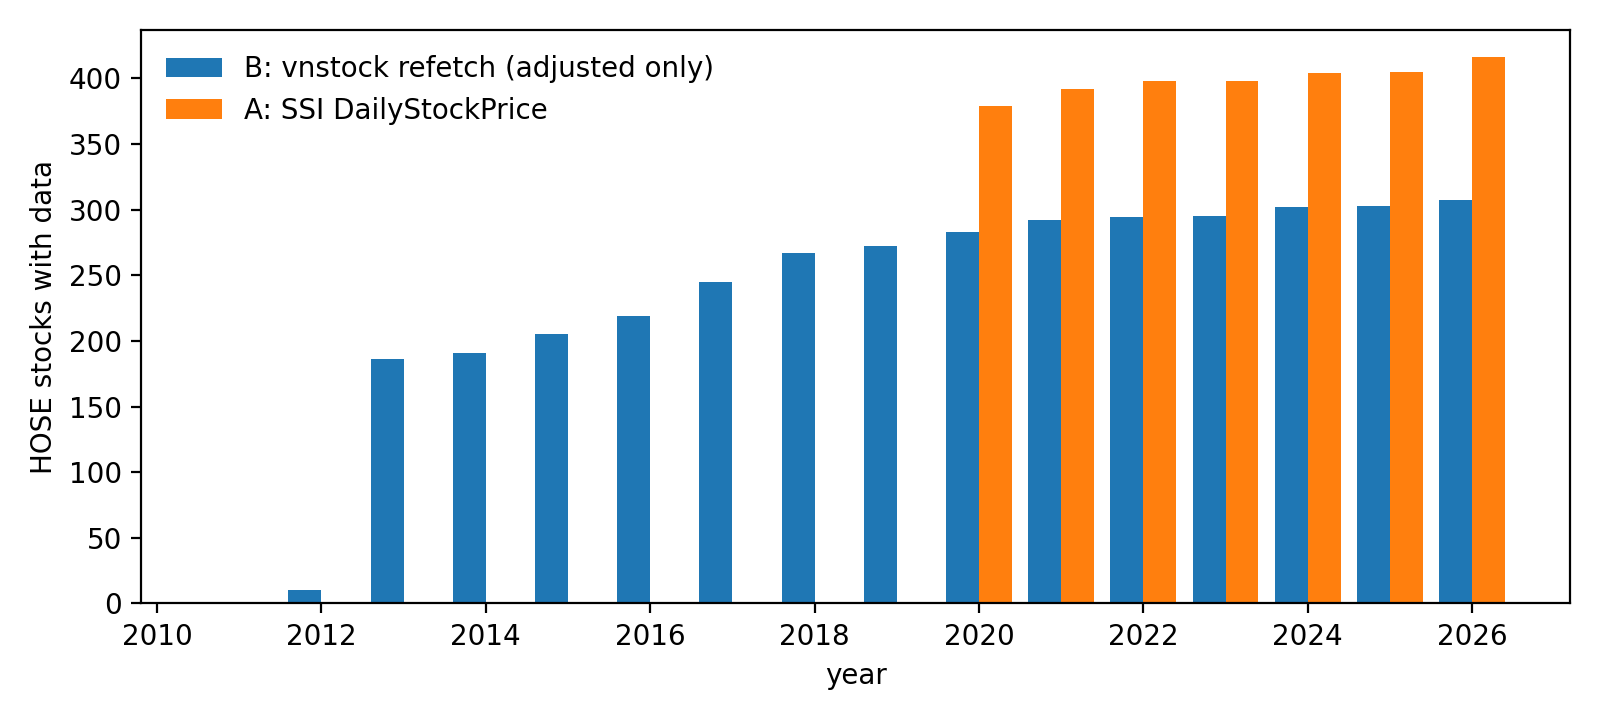
\includegraphics[width=0.85\linewidth]{figures/data_coverage.png}
  \caption{\acrshort{hose} stocks with at least one bar per year in each layer.}
  \label{fig:data-coverage}
\end{figure}

Of the 448 stocks in layer A, 140 are absent from layer B, 35 of them stocks that stopped
trading on \gls{hose} before the end of the sample. A backtest on layer B alone would
therefore only ever trade companies known, in hindsight, to have survived.

\subsection{Data Quality Findings}
\label{sec:data-quality}

Four defects were found and handled before any detector work. Each one, if left in, produces
bars that look like Wyckoff climaxes.

\begin{enumerate}
  \item \textbf{Paging duplicates.} With the \gls{api}'s default page size, pages of one query
    overlap: on average 35\% of the rows of a 30-day window were repeats while other rows were
    never served, yet the row count matched the reported total. A first build looked complete
    and held, for example, 533 bars for HPG over 6.7 years instead of about 1{,}680. Each window
    is now fetched as a single page and rejected unless its unique (ticker, date) count equals
    the reported total.
  \item \textbf{Placeholder bars on no-trade sessions.} 7.9\% of stock-sessions in layer A have
    zero matched volume. Their \gls{ohlcv} fields are placeholders (29{,}200 of the 51{,}132 are
    not even flat bars), so every such row would print a fake bar spanning the daily band. These
    sessions are kept as non-trading flags and their prices are discarded. After removing them,
    the count of opening gaps beyond $-11\%$ (impossible inside the $\pm7\%$ band without a
    corporate action) on the raw series falls from 2{,}747 to 502.
  \item \textbf{Missing reference prices.} 2{,}685 rows (2{,}576 of them traded) report a zero
    reference price; ceiling and floor are then unknown for those sessions.
  \item \textbf{Incomplete adjustment.} See Section~\ref{sec:data-adjustment}.
\end{enumerate}

\subsection{Corporate-Action Adjustment}
\label{sec:data-adjustment}

Stock dividends, bonus shares and rights issues lower the price on the ex-right date without
any change in value. On an unadjusted series these drops look like a Selling Climax. Layer A
was fetched in one day, so its adjusted close sits on a single adjustment basis.

SSI's adjusted close is correct where it adjusts: of the large ex-right sessions (exchange
reference set more than 11\% below the previous close), the adjustment factor steps on the
ex-date itself. But it adjusts only 195 of 350 such sessions, and it ignores cash dividends.
Layer B adjusts cash dividends too, which is why the two layers agree within 0.5\% on only
50\% of 2020 sessions but 87\% of 2026 sessions, while the median ratio stays at 1.00 every
year: each small dividend shifts every earlier price by a few percent. Neither layer is clean:
from 2020 on, 231 large opening gaps remain in SSI's adjusted series and 307 in layer B.

The thesis therefore computes its own back-adjustment from the exchange reference price, which
on \gls{hose} equals the previous close on every session except an ex-right date. The ratio
of the two on that date is the exact adjustment factor, taken from the exchange rather than
from a vendor's corporate-action database. In 95.3\% of sessions the ratio is exactly one; the
remaining sessions are being checked one category at a time before the series is used.

\subsection{Choice of Sample Period}

Figure~\ref{fig:data-regimes} places both layers on the VNINDEX history.

\begin{figure}[ht]
  \centering
  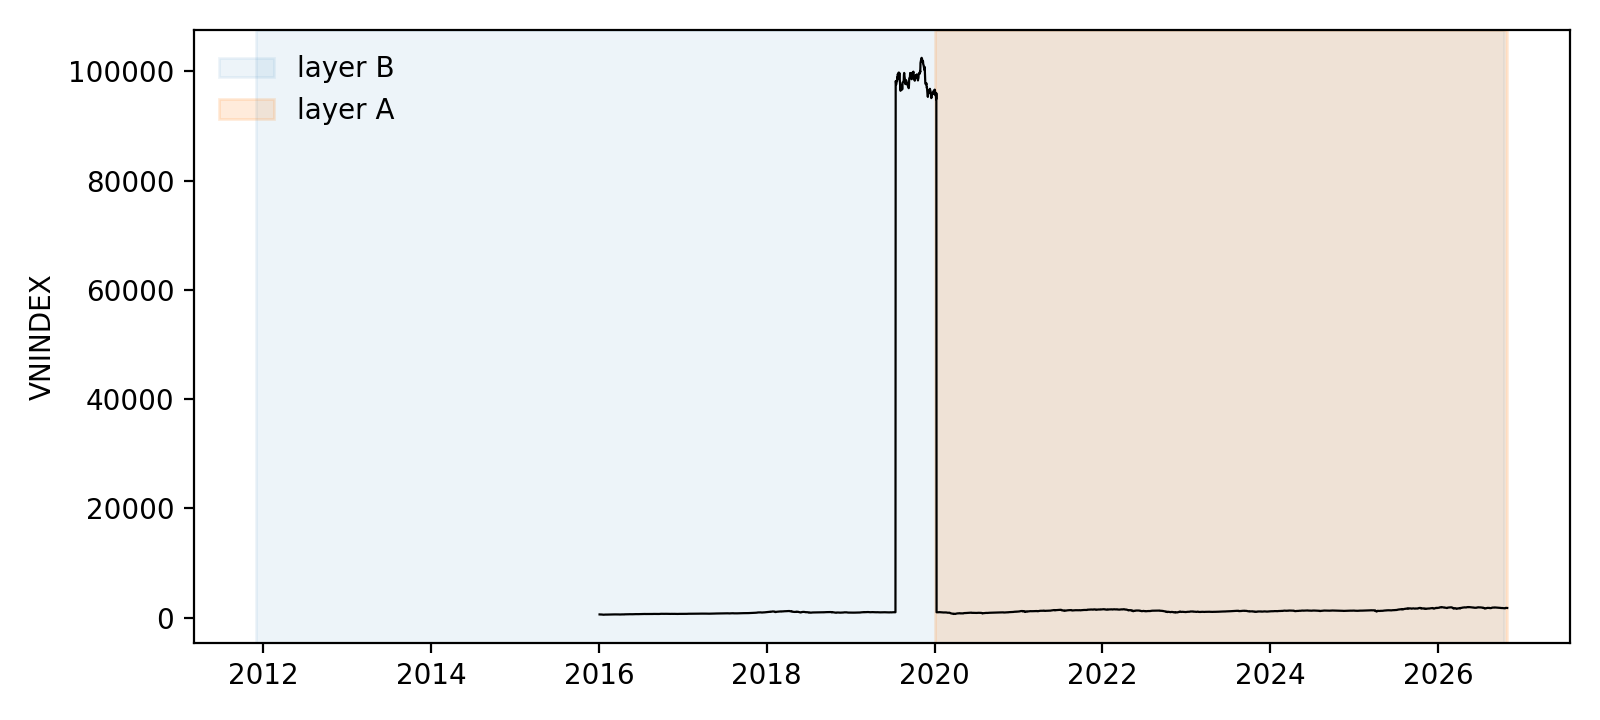
\includegraphics[width=0.85\linewidth]{figures/data_vnindex_regimes.png}
  \caption{VNINDEX and the period covered by each data layer.}
  \label{fig:data-regimes}
\end{figure}

\begin{table}[ht]
  \centering
  \caption{Start-date options.}
  \label{tab:data-period}
  \begin{tabular}{p{0.2\linewidth}p{0.36\linewidth}p{0.36\linewidth}}
    \toprule
    Option & For & Against \\
    \midrule
    Layer A, 2020-02 on (\textbf{chosen})
      & Survivorship-free; raw prices and exchange limit prices for limit-lock and execution
        modelling; foreign flow for volume confirmation; exchange reference prices allow an
        exact own adjustment
      & About 6.7 years; detector warm-up uses the first months; one full bear market (2022,
        $-40\%$) plus the COVID crash \\
    Layer B, 2013 on
      & Twice the history; adds the 2018 correction ($-27\%$)
      & Survivorship-biased; no limit prices, so limit-locks cannot be modelled; vendor
        adjustment with residual seams; no raw prices \\
    Splice B (pre-2020) + A
      & Longest series
      & Adjustment convention changes at the splice, creating a seam exactly at the join;
        bias differs before and after it \\
    \bottomrule
  \end{tabular}
\end{table}

The main sample is layer A from 26 February 2020 to 30 October 2026. It still covers three
distinct regimes: the COVID crash and recovery (2020--2021), the 2022 bear market and the
2023--2026 range. Layer B before 2020 is used only as a secondary, out-of-period robustness
check, reported with its survivorship bias stated next to every number.

\section{Wyckoff Event and Phase Definitions}
% Operational definitions for every event; table: event -> price rule -> volume rule.

\section{Detector}
\subsection{Swing Points and Trading Ranges}
\subsection{Event Rules}
\subsection{Phase Assignment}
\subsection{Hybrid Filter (ML)}
% Rules generate candidates, classifier filters them (meta-labeling).
\subsection{Look-Ahead Control}
% Every event carries start_bar and confirm_bar; decisions only use confirm_bar.

\section{Ground-Truth Annotation}
% Guideline, sampling, annotators, agreement measure.

\section{Trading Rules}
% Entries (Spring+Test, SOS->LPS/BU), exits (target, distribution signs, stops, time stop).

\section{Risk Management}
% Risk per trade, R:R floor, gap buffer for limit-lock, position/sector/liquidity caps,
% market-context exposure.

\section{Backtest Design}
% VN constraints (Appendix~\ref{app:vn-rules}), costs, walk-forward, baselines.

\section{Evaluation Metrics}
% RQ1: event precision/recall/F1 with +/-k bar tolerance. RQ2: CAGR, Sharpe, Sortino, MaxDD,
% expectancy (R), \gls{dsr}, \gls{pbo}. RQ3: per-regime and cross-engine agreement.
